
% Luigi Coniglio 
\subsection{En-tete IPv4}
Un packet IPv4 est precede` par un en-tete ayant une longeur minimale de 20 octets 
(dans les cas aucune option supplementaire a ete specifie`).
La figure suivante montre le contenu de l'en-tete d'un packet IPv4.


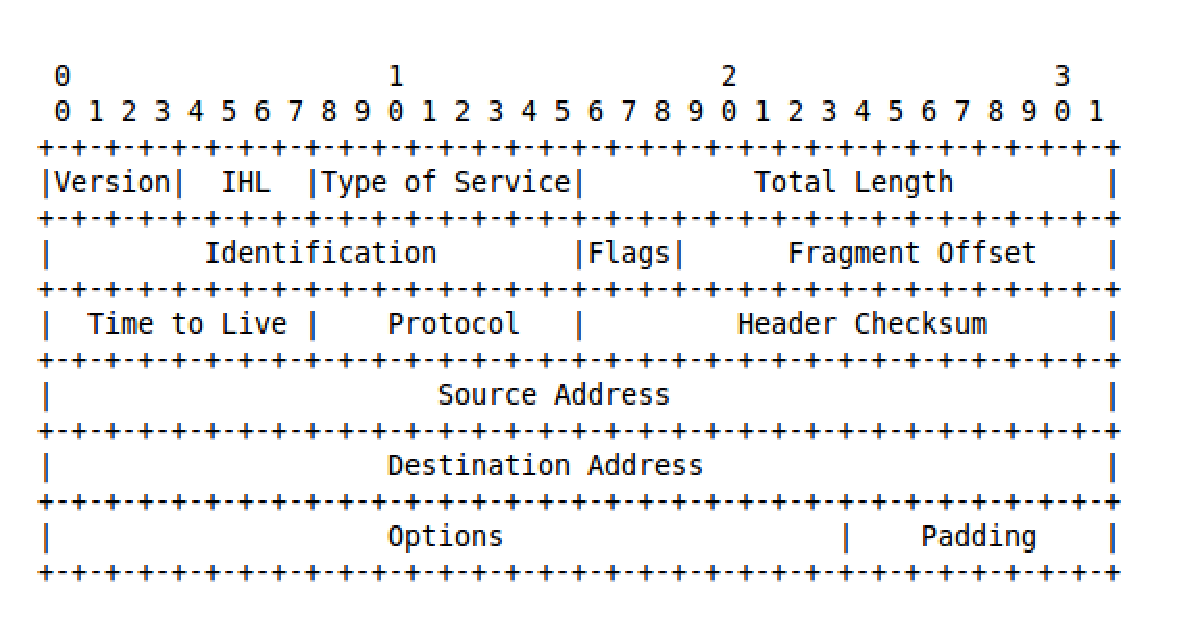
\includegraphics[width=15cm]{./pics/IPv4header.eps}


Comme on peut voir dans la figure ci dessus, un en-tete IPv4 est compose` par
13 champs, plus le padding. En realite nous verrons plus loin que cet en-tete
peut, quand il est necessaire, contenir un champ additionel qui servira a
specifier quelque option qui n'est pas presente dans le 13 champs ci dessus.


Commencons par voir plus en detail les 13 champs d'un en-tete IPv4 standard:

\begin{description}
\item [Version] 
Cette champ occupe les premiers 4 bits de l'en-tete IPv4. Il est
utilise pour determiner le type de protocole utilise` par la couche
reseau (chouche 3). Dans le cas de IPv4 cet champs contiendra toujours
la valeur 4, qui justement identifie le protocole IPv4.

La position de ce champ dans l'en-tete n'est pas casuelle. En effet pour
connaitre la positions des autres champs de l'en-tete il faut d'abord savoir
quel est le protocole utilise et donc le type de en-tete.
En pratique dans la plus part des cas cet champ n'est pas tres utile, car le
protocole a utiliser pour la couche 3 est souvent specifie dans l'en-tete du
protocol de la couche liason.

\item [IHL]
Le champ IHL specifie la taille de l'en-tete IPv4, en fait IHL est 
l'acronime de Interet Header Length. Bien entendu, en disant cela on souligne
un concept important a propos du protocole IPv4: la taille de l'en-tete n'est pas fixe.

La taille de l'en-tete est exprime`e en bloques de 32 bits. Etant donne une taille de
4 bits pour le champ IHL, la longueur maximale d'un en-tete IPv4 est de 15 bloques de
32 bits, qui correspond a 60 octets. Comme l'en-tete IPv4 a une taille minimale
de 20 octets (160 bits), le champ IHL ne peut pas contenir un valeur inferieure a 5.

\item [Type of Service]
Le champ Type of Service, mieux connu avec l'acronime ToS, est utilise pour 
specifier la qualite de service souhaite pour l'envoi d'un packet IPv4.
Cet champ occupe un octet de l'en-tete et il se compose en trois parties.
Une premiere partie de 3 bits permet d'indiquer la precedence avec la quelle
le packet doit etre traite, les 3 bits apres sont utilise pour specifier 
certaines caracteristiques du service, notament: le temp, le debit et la fiabilite.
Enfin l'emploi des 2 derniers bits n'a pas ete specifie et leur usage a ete 
laisse libre pour des implementationes futures.


En realite l'histoire de cet champs est bien plus longue et complexe que ca,
car en pratique la facon d'utiliser cet champs a ete modifie plusieurs fois au 
cours des annees.
\footnote{L'utilisation des 8 bits du champ ToS a ete redefinie
par cinq standard differents (plus divers standars experimentals).
Les documents presentent ces standard sont mentionne dans le chapitre 
"Historical Definitions for the IPv4 TOS Octet" du RFC 3168}
Cette manque de stabilite a par fois cause une certaine confusion dans les implementations.
\footnote{Comme le souligne le RFC 3260 {\it "At least one implementor has expressed confusion about the
relationship of the DSField, as defined in RFC 2474, to the use of
the TOS bits, as described in RFC 1349"}}

Aujourd'hui les 8 bits du champ ToS sont utilise par le mecanisme DiffServ
(Differentiated Services). Cet systeme utilise les premieres 6 bits du champ
ToS (DSCP - Differentiated Services Code Point) pour marquer chaque paquet
comme appartenant a un niveau de priorite et une classe de service.  Chaque
classe determine le type de traitement que on souhaite demander pour le paquet
aux routers au long du chemin (PHB - Per-Hop behaviour), toutefois le service offert
par chaque router est fortement lie a sa configuration.
\footnote {
{\it "The DiffServ standard does not specify a precise definition of "low," "medium,"
and "high" drop probability. Not all devices recognize the DiffServ (DS2 and
DS1) settings; and even when these settings are recognized, they do not
necessarily trigger the same PHB forwarding action at each network node. Each
node implements its own response based on how it is configured."} - 
Implementing Quality of Service Policies with DSCP
http://www.cisco.com/c/en/us/support/docs/quality-of-service-qos/qos-packet-marking/10103-dscpvalues.html
}}
Le dernieres 2 bits du champ ToS sont utilise pour l'extension ECN ({\it Explicit Congestion
Notification }). Cette extension, propose par RFC2481 et introduite deux annees apres avec le RFC3168,
ajoute un systeme de controle de la congestion du traffic reseau. Dans le cas d'une saturation
de la reseau cet champ est utilise pour notifier cet probleme et demander a le dispositif emetteur
une reduction du rythme au quel les packets sont envoye, avec l'objectif de reduir l'attente et
la perte de packets.

\item [Total length]
Comme le suggere le nom, ce champs est utilise pour indiquer la taille totale du
packet IPv4: en tete plus donnes. Le champ {\it Total length} est defini sur 16
bits, ceci permet de indiquer un valeur compri entre 0 et 65,535 octets. Comme l'en-tete
est compris dans la longeur totale d'un packet cet valeur ne sarait jamais inferieur
a 20 (taille minimale d'un en-tete IPv4 en octets).
RFC 791 impose a toutes les dispositifs d'une reseau IPv4 la capacite de recevoir
des packets jusq'a une taille de 576 octets, cette prerogative permet de
eviter une excessive fragmentation.

\item [Identification]
Cet en-tete (sur 16 bits) permet d'identifier les fragments appartenent au meme packet.

\item [Flags]
Le 3 bits du champs Flags sont utilise pour gerer la fragmentation d'un packet.
Un de ces bit est emploie pour indiquer si le paquet peut etre fragmente ou
non. Cet bit, appelle DF ({\it Don't Fragment}), doit etre pris en consideration
par les routers dans le chemin pour decider si un paquet trop grand pour etre
trasmis peut etre retrasmis sous forme de fragments plus petits ou rejete. 
Un autre bit, appelle MF ({\it More Fragments}), indique si le paquet est suivi 
par d'autres fragments. Le bit MF est mis a 0 dans le dernier fragment ou dans
des paquet qui n'ont pas ete fragmente.

Un des trois bits de ce champs n'est pas actuallement utilise mais il a ete
reserve pour applications futures possibles.
\footnote {Cet bit a ete aussi le protagoniste d'un des plus connu poissons
d'avril presentee par le IETF. Pour faciliter les taches des systems de filtrage 
le RFC 3514 propose d'utiliser ce bit pour etiqueter paquets mailveillant, a ce
titre tous les paquets etant envoye avec ce bit (renomme "{\it Evil Bit}") 
mis a 1 seront mis a la poubelle.
}

\item [Fragment Offset]
Lorsque un paquet a ete fragmentee cet en-tete est utilisee pour determiner la 
position (offset) d'un fragment par rapport a les donnees du paquet reassemble.
Le decalage de chaque fragment est exprime en bloques de huit octets (ou 64
bits).  Le champ Fragment Offset utilise 13 bits de l'en-tete IPv4, cela permet
un offset maximale de 65,528 octets.\footnote {En pratique un tel offset n'est
jamais utilisee car, en ajoutant un en-tete minimale de 20 octets, la taille 
totale du paquet reassemble depaserait la longeur maximale d'un paquet IPv4.}
Etant donne que la flag MF ({\it More Fragments}) doit etre mise a zero lorsque 
si un paquet n'est pas fragmentee ou si il est le dernier fragment d'un paquet
plus grand, l'unique difference entre ce deux types de paquets est le valeur
de le champ Fragement Offset que, dans le cas d'un paquet pas fragmentee, est
toujours zero.

\item [Time to Live]
Cet champ determine le nombre maximal de fois qu'un paquet peut etre retrasmis, 
il est utilise pour empecher que un paquet puisse etre retrasmis a l'infini.
Chaque router au long du chemin d'un paquet est tenu a detruir un paquet si le
valeur du TTL ({\it Time to Live}) est zero ou decrementer cet champs par le
nombre de secondes que le paquet passe en attente d'etre trasmis.

En theorie le TTL indique le nombre de secondes pendant le quels un paquet
peut continuer a etre retrasmis dans une reseau ,mais , etant chaque router
toujour tenu a decrementer cet champ de au moins 1 (meme si le paquet a ete
retrasmis en moin qu'un seconde) et considerant les performances des routers
d'aujourd'hui, en pratique le TTL indique le nombre maximum de router que
un paquet peut incontrer au long de son chemim.

Le space reservee au TTL dans l'en-tete IPv4 est de un octet ce que comporte un 
TTL maximum de 255.\footnote {Le RFC 1700 recommende un valeur par defaut de 64.}

Quand un paquet a ete detruit ensuite a l'expiration du TTL, le router qui a
detruit le paquet peut decider de envoier un message d'erreur a l'emetteur du
paquet detruit. Cet type de message (ICMP Time exceeded) est utilise par
utils comme {\it traceroute} pour decouvrir, approximativement, le chemin 
d'un packet IP.

\item [Protocol]
Chaque paquet IPv4 specifie le protocole utilise par les donnes trasmises:
cela est l'objectif de ce champs de 8 bits 

\item [Header Checksum]
Cet champ contient une somme de controle et est utilise pour detecter des 
erreurs dans l'en-tete IPv4. Le valeur de cet champs est recalcule at
chaque retrasmission\footnote {Cela est necessaire car le TTL est decrementee
at chaque retrasmission et un changement de l'en-tete comporte un valeur different
dans la somme de controlle}: si il ne correspond pas avec celui 
presente dans l'en-tete le paquet est detruit.


\item [Addresse source et Addresse destination]
Les addresses de chaque paquet IPv4 (soit l'adresse source que l'adresse de
destination d'un paquet) sont represente sous forme d'une suite de 32 bits.

L'addresse source de chaque packet represente dans la plus part des cas
l'addresse logique\footnote {Il ne faut surtout pas oublier la difference entre
un addresse physique, comme par example un addresse MAC (qui est lie a
l'hardware et est donc unique pour chaque machine), et un addresse logique,
comme par example un addresse IP (qui peut changer et identifie une machine
dans une reseau en particuliere).} de la machine qui a envoye le paquet
(a laquelle il faudra eventuellement repondre donc).  Dans certains cas
specifiques cette addresse ne correspond pas a celui de la machine qui a envoye
le paquet, c'est par exemple ce qui se passe dans une requete {\it ARP probe}
la ou le valeur de l'adresse de la machine source est 0.0.0.0 (ce qui represente
un adresse indefini\footnote {Notex que la signification de l'adresse 0.0.0.0
est lie a la facon dont il est utilise. En general il indique {\it aucune
adresse en particulier}.  Dans la plus part des cas cet adresse est utilise
pour indiquer un de ces valeurs: l'adresse de la machine courant (c'est
l'adresse de loopback), n'importe quel adresse ou reseau (c'est le cas de la
route par default dans une table de routage), un adresse indefini ou bien une
combinaison des possibilites precedentes (c'est le cas d'une requete {\it ARP
probe} ou bien d'une requete {\it DHCP Discovery} ou {\it DHCP Request}, ou en
fait l'adresse source 0.0.0.0 indique un adresse indefinie mais aussi l'adresse
de la machine actuelle, que del reste n'est pas encore defini...).}
) car elle n'a pas encore determine son addresse IP. 

L'addresse de destination d'un paquet IPv4 identifie la machine vers
laquelle le paquet doit etre expedie. Comme dans le cas de l'adresse source,
aussi l'adresse destination peut contenir des valeur speciaux. En effet certains 
valeurs puvent etre utilise par example pour identifier plusieurs machines
(adresses multicast), toutes le machines d'une reseau (adresse de broadcast) ou
la machine actuelle (adresse de loopback).

Une description plus detaile des mechanismes lies aux adresses IPv4 est
propose dans le chapitre 
%TODO mettre chapitre% 
de ce rapport.


\item [Options] 
Cet champ n'est pas obligatoire et donc il peut ne pas etre present dans un
en-tete IPv4. La presence de cet champ est determine par le valeur du
IHL: lorsque cette valeur indique une taille de l'en-tete IPv4 superieure a 
la taille minimale (20 octets), l'en-tete contiens des options.
Etant donne que un en-tete IPv4 peut avoir une taille maximale de 
60 octets (le valeur du IHL est egal a 15), le champ Options peut occuper
40 octets au meximum.

Ce champ est ne pour etendre les possibilites de IPv4 en ajoutant des fonctions extra.
Aujord'hui il y a quelque dizaine de options qui ont ete specifie\footnote
{http://www.iana.org/assignments/ip-parameters/ip-parameters.xhtml} (si on
considere aussi les options experimentales) mais peu entre eux sont reelement
utilise. 
Entre les options les plus connues on retrouve par example des ajoutes
utiles a l'administration et au debouggage d'une reseau, comme {\it Record route}
qui permet de enregistrer les addresses des routeurs dans le chemin d'un 
paquet IP, et {\it Timestamp} qui permet de savoir le temp passe 
entre chaque hop du chemin.

Entre les options il en y a deux qui ont une fonction speciale: EOL 
({\it End Of Option List}) and NOP ({\it No Operation}): l'option EOL 
est utilise pour indiquer la fin de la chaine d'options, NOP est une option
sans aucun effet, elle est utilise comme replissage pour aligner les options 
quand elles ne sont pas aligne sur 4 octets\footnote {On rappelle que 
le champ IHL indique la longuer de l'en-tete IPv4 en bloques de 32 bits 
(4 octets)}.



\item [Padding] 
Le padding ne contiens que des zeros et est utilise quand la fin de l'en-tete
n'est pas aligne sur 32 bits (4 octets). Bien entendu, cet champ est optionel:
en effet il pest etre necessaire seulement lorsque l'en-tete IPv4 termine avec
une option lequel limite n'est pas aligne sur 32 bits. Un en-tete n'a besoin
d'aucun Padding standard IPv4 de 20 octets (donc sans aucune option) termine
comme etant aligne sur 4 octets (20 est un multiple de 4).

\end{description}
